\documentclass{article}
\usepackage{fancyhdr} % Required for custom headers
\usepackage{lastpage} % Required to determine the last page for the footer
\usepackage{extramarks} % Required for headers and footers
\usepackage{graphicx} % Required to insert images
%\usepackage{lipsum} % Used for inserting dummy 'Lorem ipsum' text into the template
\usepackage{amsmath}
%\usepackage{amsfont}
%\usepackage{amssymb}

\usepackage{multicol}
% Margins
\topmargin=-0.5in
\evensidemargin=0in
\oddsidemargin=-0.5in
\textwidth=7.5in
\textheight=9.0in
\headsep=0.25in 


\pagestyle{fancy}

\rhead{Niloufer King} % Top right header
\lhead{Rice}
\chead{ }
%\title{}

\begin{document}
%
%PRELIMINARIES:
%
%
%Begin by preheating the oven to 350 $^o$F
%
%\bigskip
%
%\bigskip

\begin{multicols}{2}
Ingredients:
\begin{itemize}
\item 1-3/4 cups of water
\item 1 cup of rice
\item A bit of olive oil or butter
\item Salt
\end{itemize}
\columnbreak

Directions:
\begin{enumerate}
\item Rinse the rice in a few changes od cold water.

\item Drain the rice well in a sieve.

\item In a medium heavy-bottomed pot with a tight-fitting lid, combine :
\begin{itemize}
\item 1-3/4 cups of water
\item 1 cup of rice
\item A bit of olive oil or butter
\item Salt
\end{itemize}

\item Bring to a boil over high heat

\item As soon as the water is boiling lower the heat to a simmer and cover.

\item Cook at a gentle simmer until the water is completely absorve and the rice is tender(~ 12 mins).

\item Remove the pot from the heat and let it sit(> 5 < 30 mins).
\end{enumerate}




\end{multicols}



\begin{center}
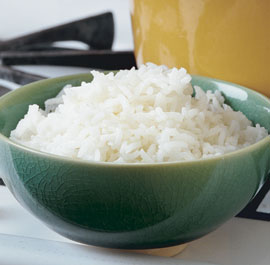
\includegraphics[scale=0.4]{rice.jpg}
\end{center}


\end{document} 











